\subsubsection{Mobility data}

\paragraph{Analysis of available datasets}

As already described in Milestone 2, we had four data sets suitable for this sector. These were two data sets on international flight activity and two mobility data sets from Google and Apple. The aviation data sets could not be used for this sector, as the number of flights was not stated explicitly for every country. We then decided to take a closer look at the Apple mobility data set, as it was easy to handle but still contained all necessary information. For every country, it contains \textit{walking} and \textit{driving} mobility data and wherever available, \textit{transit} mobility data as well. We had to pre-process this dataset a little by grouping the data of 26 out of 28 EU countries (Cyprus and Malta were not available). Furthermore, we applied a 7-day \textit{moving average} filter, to account for changes throughout the week. Unfortunately, we could not gather mobility data for China, as it was neither in the Apple mobility data set nor in the Google mobility data set. This can be directly attributed to China's restrictive handling of sensitive data. We also tried to gather information from \textit{Baidu Maps}, China's \textit{Google Maps} equivalent so-to-say. However, this proved to be very difficult, as the files are prepared in Chinese and nobody in our team is able to read Chinese. Therefore, we had to calculate China's mobility indicator from other countries' mobility data and do a few assumptions.

\paragraph{Data visualization}

As it is interesting to see the drop in international flights, we depicted it in \autoref{fig:flights}. In \autoref{fig:driving} and \ref{fig:transit}, we show the raw, unprocessed data and our result after applying a moving average filter. From the two figures, we can see that \textit{driving} mobility almost recovered to a normal level for most countries, while \textit{transit} mobility is still low for all countries except Japan.


\begin{figure}[hb!]
	\centering
	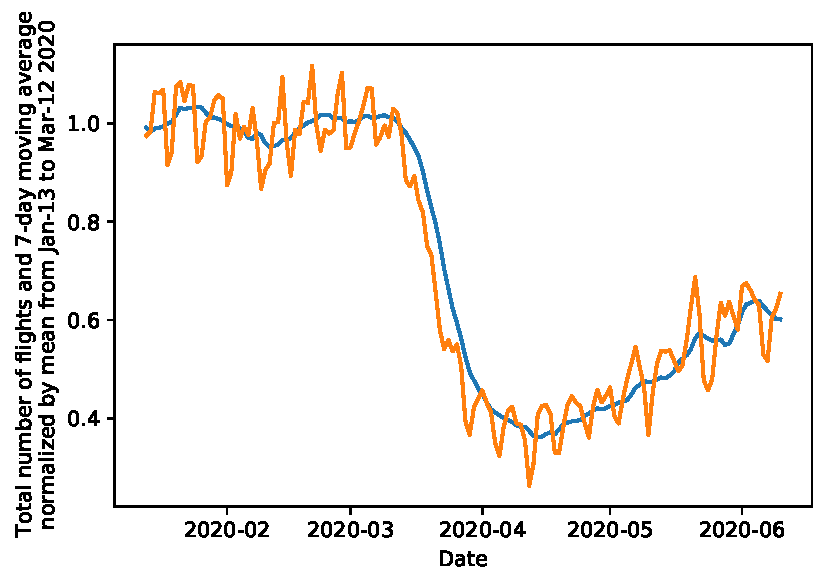
\includegraphics[width=0.7\linewidth]{../predictions/flights.pdf}
	\caption{International flights data.}
	\label{fig:flights}
\end{figure}


\begin{figure}[h!]
	\centering
	\subfloat[Raw driving data]{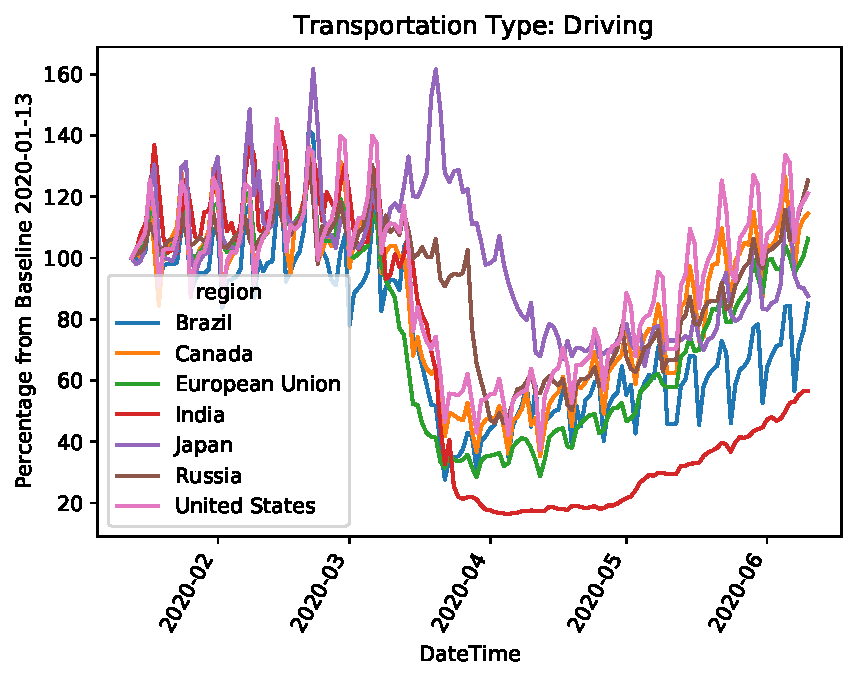
\includegraphics[width=0.48\linewidth]{../predictions/driving.pdf}}
	\hfill
	\subfloat[Driving data with moving average]{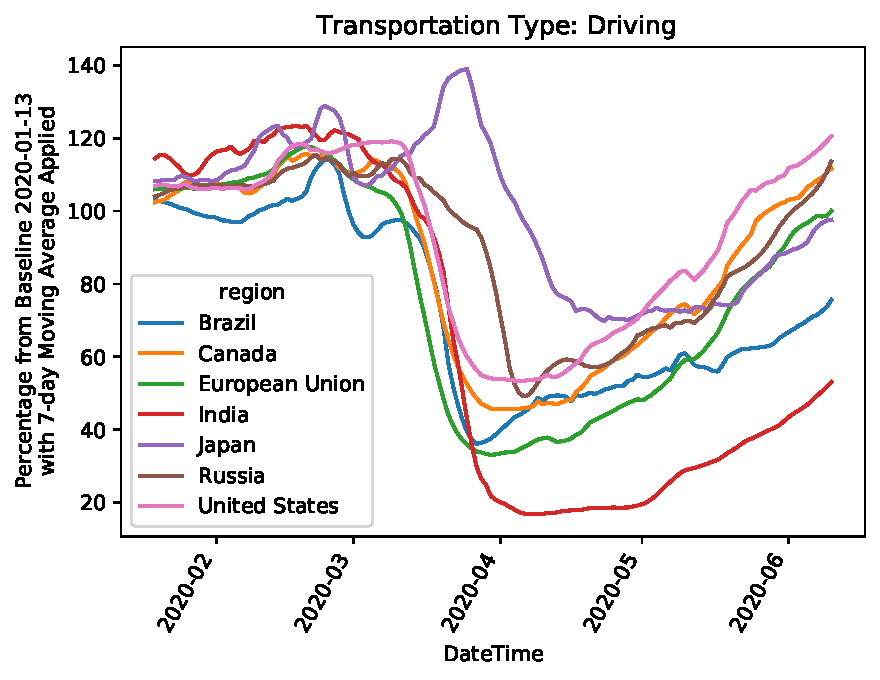
\includegraphics[width=0.48\linewidth]{../predictions/driving_ma.pdf}}
	\caption{Mobility data. A steep drop is visible for all countries.}
	\label{fig:driving}
\end{figure}

\begin{figure}[h!]
	\centering
	\subfloat[Raw transit data]{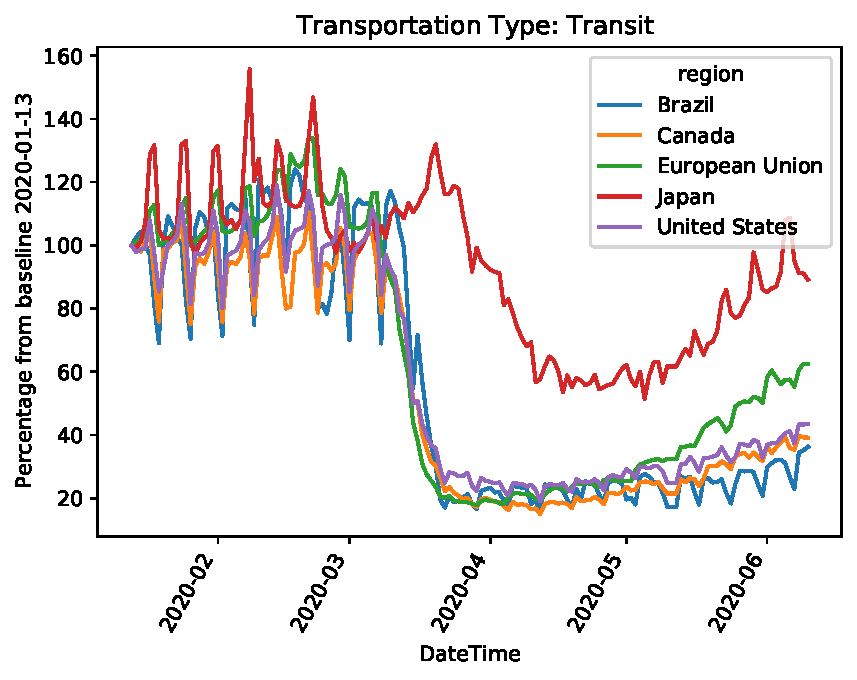
\includegraphics[width=0.48\linewidth]{../predictions/transit.pdf}}
	\hfill
	\subfloat[Transit data with moving average]{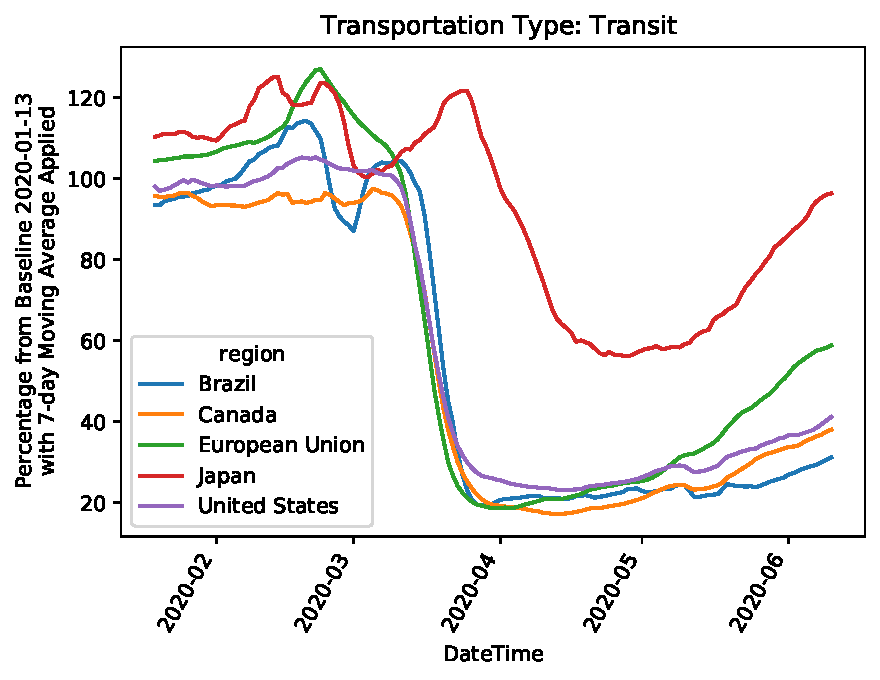
\includegraphics[width=0.48\linewidth]{../predictions/transit_ma.pdf}}
	\caption{Mobility data. A steep drop is visible for all countries that transit data was available for.}
	\label{fig:transit}
\end{figure}

\paragraph{Result}

Due to the huge size of the project, we had to cut back on some details and make some assumptions. As we could not find out the correct contributions of transit and driving mobility to the \co emissions of this sector, we had no choice but to weigh those two categories equally. We then calculated the monthly average, which lead to the resulting indicators depicted in \autoref{fig:indicator_mobility}. As all data is normalized to the first day of available data, all indicators should start at one. But since we are taking the mean of the first month, one can see small deviations from one for most countries.

For China, we had to assume a curve similar to the others and took mean values of suitable countries and set the mobility to one in months were COVID-9 had no to little impact, like January and June.


\begin{figure}[ht!]
	\centering
	\subfloat[Transit indicator]{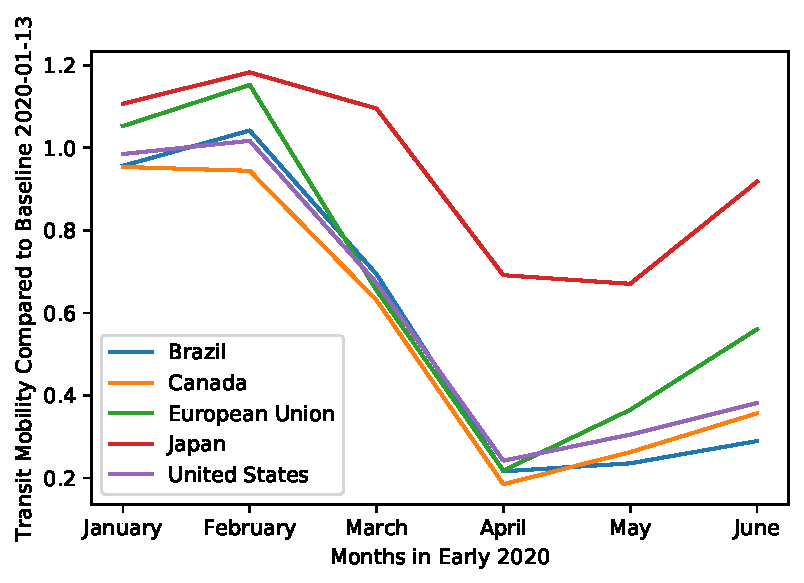
\includegraphics[width=0.48\linewidth]{../predictions/indicator_transit.pdf}}
	\hfill
	\subfloat[Driving indicator]{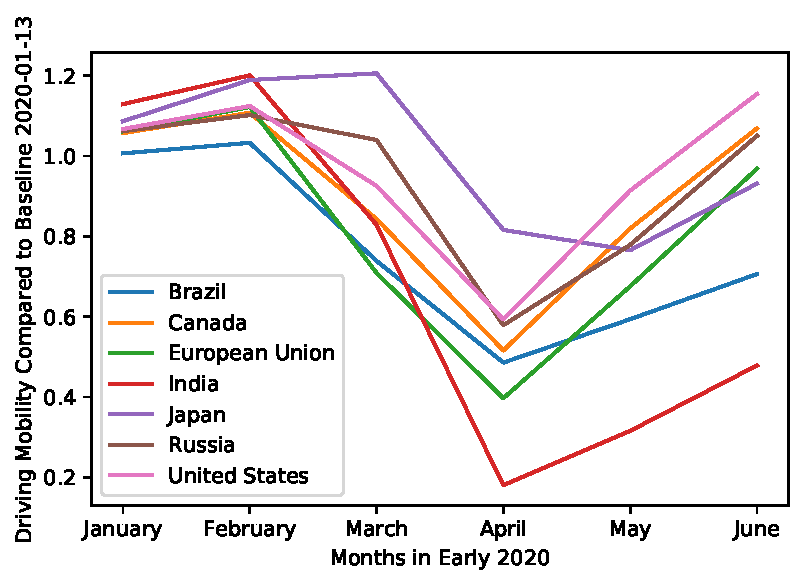
\includegraphics[width=0.48\linewidth]{../predictions/indicator_driving.pdf}}
	\caption{The two \textit{driving} and \textit{transit} mobility indicators before we combine them to one overall mobility indicator.}
	\label{fig:both_mobility_indicators}
\end{figure}

\begin{figure}[hb!]
	\centering
	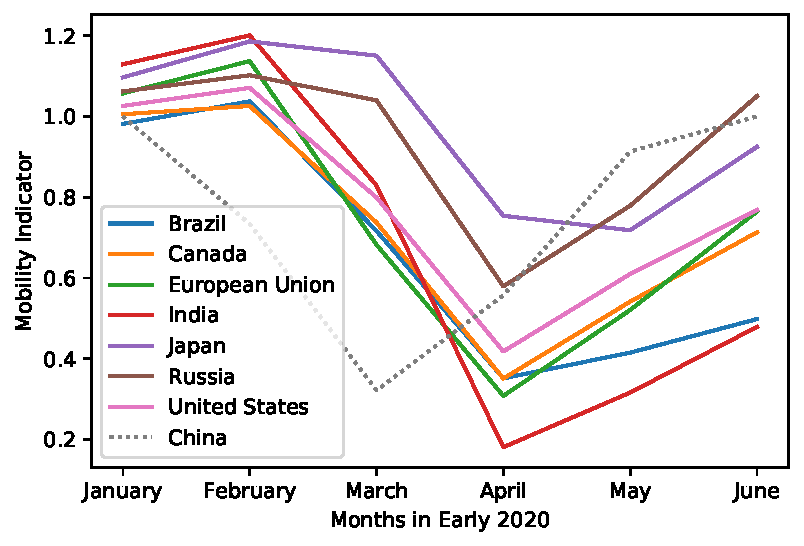
\includegraphics[width=0.7\linewidth]{../predictions/full_mobility_indicator.pdf}
	\caption{Calculated mobility indicator, including China.}
	\label{fig:indicator_mobility}
\end{figure}

\paragraph{Conclusion}

It is very unfortunate that we have no data on China, as it is the biggest emitter of \co. This definitely has an impact on the validity and accuracy of the mobility indicator and therefore the model. Still, we tried to model China's mobility as accurately as possible. As we can see in \autoref{fig:indicator_mobility}, we assume that China's emission drop earlier than the others, which is a fair assumption as the pandemic started in China.